\documentclass[a4paper]{article}

% Pacotes para o português.
\usepackage[brazilian]{babel}
\usepackage[utf8]{inputenc}
\usepackage[T1]{fontenc}

\usepackage{sbc-template}

\usepackage{datetime}
\usepackage{graphicx}
\usepackage{float}
\usepackage{indentfirst}
\usepackage{amssymb}
\usepackage{multirow}
\usepackage[nottoc]{tocbibind}

% Espaçamento duplo.
\usepackage{setspace}
 % Breaklines nas citações.
\usepackage{cite}

% Linha horizontal.
\newcommand{\HRule}{\rule{\linewidth}{0.5mm}}
\newcommand{\hRule}{\rule{4.5cm}{0.1mm}}

% Listagens.
\newfloat{program}{thp}{lop}
\floatname{program}{Listagem}

% Figuras.
\newcommand{\figurex}[5]
{
\begin{figure}[htb, h!]
   	\setlength{\unitlength}{1.0cm}
   	\centering
   	\includegraphics[scale=#1]{./img/#2.#3}
	\begin{center}
	   	\parbox{.9\linewidth}{\footnotesize \sf \caption{#5}  \label{#4}}
	\end{center}
\end{figure}
}

\newcommand{\ck}[0]
{
\checkmark
}

\hyphenation{}

\begin{document}

%\doublespacing
\onehalfspacing

\begin{titlepage}
\begin{center}

% Topo 1.
\textsc{\Large UNIVERSIDADE FEDERAL DE ITAJUBÁ\\
	INSTITUTO DE MATEMÁTICA E COMPUTAÇÃO}\\[0.7cm]

% Topo 2.
\textsc{DEPARTAMENTO DE MATEMÁTICA E COMPUTAÇÃO}\\[2.8cm]

% Título.
\textsc{\Large Seminário}\\
\HRule \\[0.4cm]
{\Large \bfseries Arquitetura Peer to Peer}
\HRule \\[0.4cm]
\textsc{REDES DE COMPUTADORES}\\[2.8cm]

% Etc.
\begin{minipage}{0.4\textwidth}
\begin{flushleft} \large
\emph{Alunos:}\\[0.43cm]
%\hRule\\
David Mateus Batista\\
Gabriel Erzinger Dousseau\\
Gabriel Alves Taets\\
Mauricio Leite\\
\end{flushleft}
\end{minipage}
\begin{minipage}{0.4\textwidth}
\begin{flushright} \large
\emph{Professor:}\\[0.4cm]
%\hRule\\
Bruno Guazzelli Batista
\end{flushright}
\end{minipage}

\vfill

\today

\end{center}
\end{titlepage}

\thispagestyle{empty}

\section*{Resumo}
Esta monografia tem o objetivo de estudar e analisar a arquitetura de redes Peer-to-peer,
suas vantagens, desvantagens, limitações e aplicações.
\newpage
\pagenumbering{Roman}

\tableofcontents
\newpage
\pagenumbering{arabic}

%http://www.fio.edu.br/manualtcc/co/1_Estrutura_do_TCC.html%
\section{Introdução}
\newpage

\section{Fundamentação Teórica}
\newpage

\section{Aplicações}
Como visto nas seções anteriores, a utilização da arquitetura \textbf{P2P} pode trazer diversas vantagens, desvantagens e outras características únicas para o aplicativo ( ou serviço ) que estará implementando-a. \\
Dessa forma, é importante analisar quais serviços utilizam essa arquitetura, como se beneficiam de suas vantagens e como lidam com suas desvantagens. Isto é, dissecar sobre como as caracteristicas da arquitetura P2P são tratadas em cada caso de uso.
\subsection{Napster}
O \textbf{Napster} foi uma das primeiras aplicações de compartilhamento de arquivos, elaborada em Junho de 1999. O serviço permitia apenas o compartilhamento de arquivos \textbf{MP3} e é um grande responsável pela popularidade do termo "P2P".
\subsubsection{Funcionamento}
A aplicação se basea num servidor central de indices. Os nós da rede registram uma lista dos arquivos que desejam compartilhar. Dessa forma, a busca é processada baseando-se em \textbf{palavras chave} e retornará uma lista com os arquivos encontrados e informações como a banda disponivel, tamanho e fonte. \

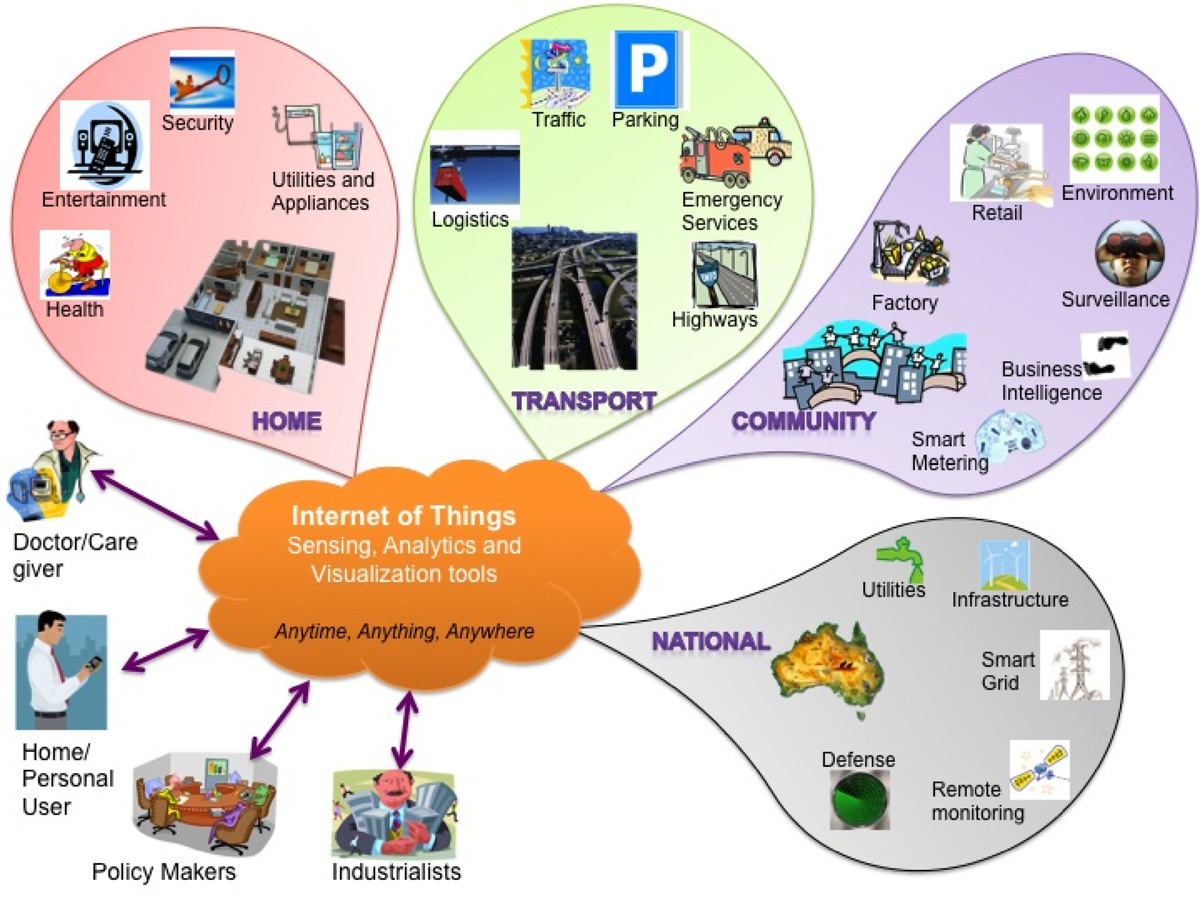
\includegraphics[width=\linewidth\center]{img//ilustracaoiot.png}

Dessa forma, o usuário fazia uma requisição de busca nos índices do servidor centralizado e obtinha uma lista de nós que possuiam aquela informação, para depois, trocar arquivos com estes nós.
\subsubsection{Vantagens e Desvantagens}
Como um dos pioneiros na área, a principal vantagem do Napster se devia ao fato de ele possuir uma busca rápida e eficiente ( por se tratar apenas de uma consulta ao servidor central ). Além disso, oferecia uma visão simples e consistente da rede. \
As desvantagens se devem exatamente a \textbf{presença de um servidor}, uma vez que, assim como em arquiteturas cliente-servidor, a central representa um ponto de falha único, que se fosse afetado, prejudicaria toda a rede. Por se tratar de um servidor que lida com diversas requisições, o servidor central também possuia um alto custo de manutenção.
\subsection{Gnutella} %https://pdfs.semanticscholar.org/f0b5/86bda8901c2f3ae399b48239690028f69417.pdf
%https://pt.slideshare.net/uschmidt/peertopeer-systems/7-P2P_Filesharing_The_most_popular
Gnutella é um \textbf{protocolo de busca} aberto e descentralizado usado principalmente para o compartilhamento e a busca de arquivos. Foi criado com o objetivo de ser uma rede dinamica que permite que seus usúarios entrem e saiam a qualquer momento, tenha uma boa escalabilidade, garanta a anonimidade  e confiança em relação a ataques externos.
\subsubsection{Funcionamento}
O termo Gnutella se refere a todo o grupo de computadores que possuem aplicativos carregados com o protocolo Gnutella que formam uma espécie de rede virtual. Cada nó nessa rede pode funcionar tanto como um cliente como quanto um servidor. \\
Dessa forma, eles podem criar e receber requisições com outros nós utilizando os dados que estarão em seu disco rígido. Como é sábido, tais requisições não são enviados para nenhum servidor central, elas são exclusivamente tratadas entre os nós da rede.
\subsubsection{Mecanismo de Busca}
O protocolo utiliza o algoritmo padrão conhecido como BFS( \textbf{B}readth \textbf{F}irst \textbf{S}earch) - Busca em Largura - portanto, tal qual o algoritmo é utilizado em grafos, ele será utilizado na rede de aplicativos que utilizam o protocolo:
\begin{itemize}
	\item O nó inicialmente busca um arquivo e envia a mensagem de busca a seus vizinhos
	\item Os vizinhos encaminham a mensagem para todos os seus vizinhos
	\item Os Nós que possuirem o arquivo que está sendo requisitado, começam uma mensagem de resposta
	item Após a mensagem de resposta atingir o nó origem, o download do arquivo começa.
\end{itemize}
\subsubsection{Mecanismo de Download}
Uma conexão é estabelecida entre a origem e o nó que possui a informação necessária. O download de arquivos sempre funciona fora da rede e faz-se o uso do protocolo HTTP para tal conexão.
\subsubsection{Desvantagens}
As desvantagens da utilização do protocolo Gnutella claramente deriva das desvantagens da própria arquitetura P2P. Portanto, temos como as principais desvantagens:
	\begin{itemize}
		\item Grande parte dos arquivos é oferecido/servido por uma pequeníssima parte dos nós, dessa forma, a rede pode acabar se tornando \textbf{quase} como uma rede cliente-servidor.
		\item Perca de banda e segurança de rede devido a transferência de arquivos.
		\item Problemas com usuários maliciosos.
		\item A busca, diferente do aplicativo anterior, pode levar um considerável periodo de tempo, visto que é necessário propagá-la nó a nó.
	\end{itemize}

\newpage

\section{Discussão}
\newpage

\section{Considerações finais}
\newpage

%*********************************************************************************************
\newpage
\bibliographystyle{apalike}
\bibliography{bibliography}

\end{document}
